\chapter{Implementácia}\label{chap:implementation}
V tejto kapitole sa zameriame na riešenie popísanej problematiky, implementáciu algoritmov a funkcií potrebných na správnu funkčnosť a dosiahnutie cieľov zadania diplomovej práce. Implementácia pozostáva z dvoch hlavných častí. Vytvorenie synchronizačného servera a klientskej aplikácie grafického editora formou rozšírenia systému MediaWiki. Popíšeme si ich dátové modely a funkcionalitu. 

Pri implementácií využívame verziovací systém GIT. Obe hlavné časti sú umiestnené vo vlastných repozitároch na serveri GitHub. 

\section{Synchronizačný server}
Synchronizačný server pozostáva z JavaScriptovej aplikácie naprogramovanej v jazyku JavaScript. Aplikácia je spúšťaná v runtime prostredí NodeJS servera, konkrétne vo verzii 7.6 a vyššej. Ten je nainštalovaný formou kontajnerového systému docker. Aplikácia pracuje pomocou inštancie HTTP servera, využívajúceho port s číslom \code{8080} a lokálnu adresou servera \code{0.0.0.0}. 

Knižnice servera sú inštalované pomocou balíčkovacieho manažéra NPM (\textbf{N}ode \textbf{P}ackage \textbf{M}anager). Ich potrebné verzie sú zapísané v súbore \code{package.json}. Nachádzajú sa tu taktiež konfiguračné premenné prostredia:

\begin{itemize}
	\item \code{api_endpoint} -- adresa API koncového bodu systému MediaWiki, v ktorom je nainštalované naše rozšírenie. V našom prípade má hodnotu \code{\"https://wiki.matfyz.sk/api.php\"}.
	
	\item \code{api_token} -- tajný token slúžiaci na overenie pripájaných klintov. Jeho hodnota sa musí zhodovať s hodnotou na strane rozšírenia.
\end{itemize}

\subsection{Dátový model}
Pre implementáciu serverovej časti aplikácie využívame dátovú štruktúru JavaScriptových objektov.

\subsubsection{User}
Trieda \code{User} reprezentuje používateľa pripojeného na synchronizačný server. Jej vlastnosti určujú triedne premenné a metódy opísané v tabuľkách \ref{tab:server-prop-user} a \ref{tab:server-func-user}.

%\begin{description}[style=nextline]
%	\item[name] Meno používateľa prijaté v dopyte pri pripojení klienta na server.
%	\item[color] Automaticky generovaná farba pomocou funkcie \code{getRandomColor()} v hexadecimálnom formáte {\code{\"#ffff00\"}}.
%	\item[verified] Príznak, či bol korektne overený bezpečnostný token.
%	\item[token] Privátna premenná s hodnotou bezpečnostného tokenu.
%\end{description}
%

\begin{table}
	\begin{tabular}{ | m{3cm} | m{3cm}| m{6.5cm} | } \hline
		\textbf{Názov} & \textbf{Typ} & \textbf{Popis} \\ \hline \hline
		
		name & string & Meno používateľa prijaté v dopyte pri pripojení klienta na server. \\\hline
		color & string & Automaticky generovaná farba pomocou funkcie \code{getRandomColor()} v HEX formáte {\code{\"#ffff00\"}}. \\\hline
		verified & boolean & Príznak, či bol korektne overený bezpečnostný token. \\\hline
		token & string & Privátna premenná s hodnotou bezpečnostného tokenu. \\\hline
		
		\hline
	\end{tabular}
	\caption{Zoznam triednych premenných objektu User}
	\label{tab:server-prop-user}
\end{table}


\begin{table}
	\begin{tabular}{ | m{4cm} | m{8.5cm} | } \hline
		\textbf{Názov} & \textbf{Popis} \\ \hline \hline
		
		setToken(token) & Nastavenie bezpečnostného tokenu.  \\\hline
		getToken() & Vráti hodnotu bezpečnostného tokenu. \\\hline
		verifyUser() & Overí hodnotu bezpečnostného tokenu a nastaví triednu premennú \code{verified}. \\\hline
		
		\hline
	\end{tabular}
	\caption{Zoznam metód objektu User}
	\label{tab:server-func-user}
\end{table}


\subsubsection{Message}
Objekt \code{Message} reprezentuje správy odoslané používateľmi pomocou chatu v editore. Popis vnútornej reprezentácie vlastností objektu môžeme vidieť v tabuľke \ref{tab:server-prop-message}.

\begin{table}
	\begin{tabular}{ | m{3cm} | m{3cm}| m{6.5cm} | } \hline
		\textbf{Názov} & \textbf{Typ} & \textbf{Popis} \\ \hline \hline
		
		from & User & Odosielateľ správy. \\\hline
		to & User & Prijímateľ správy. \\\hline
		text & string & Textový obsah správy. \\\hline
		type & string & Typ správy nastavovaný ak ide o systémovú správu. \\\hline
		time & string & Dátum a čas odoslania správy. \\	\hline
	
		\hline
	\end{tabular}
	\caption{Zoznam triednych premenných objektu Message}
	\label{tab:server-prop-message}
\end{table}



\subsubsection{Room}
Trieda \code{Room} slúži na udržiavanie stavu miestnosti pripojených používateľov, spracovanie požiadaviek odosielaných zo strany editora, udržiavanie štruktúry objektov, odoslaných správ a funkcionality na načítanie informácií o súbore. Popis jej vnútornej štruktúry a poskytovanej funkcionality môžeme vidieť v tabuľkách \ref{tab:server-prop-room} a \ref{tab:server-func-room}.

\begin{table}
	\begin{tabular}{ | m{3cm} | m{3cm}| m{6.5cm} | } \hline
		\textbf{Názov} & \textbf{Typ} & \textbf{Popis} \\ \hline \hline
	
		users & array<User> & Zoznam používateľov. \\\hline
		messages & array<Message> & Zoznam správ. \\\hline
		objects & array<object> & Zoznam objektov grafickej plochy. \\\hline
		canvas & object & Dynamický objekt s nastaveniami grafickej plochy. \\\hline
		format & string & Formát editovaného súboru (jpg, png, svg).\\\hline
		loaded & boolean & Príznak, či je miestnosť plne vyinicializovaná. \\\hline
		file & string & Názov editovaného súboru. \\\hline
	
		\hline
	\end{tabular}
	\caption{Zoznam triednych premenných objektu Room}
	\label{tab:server-prop-room}
\end{table}


\begin{table}
	\begin{tabular}{ | m{6cm} | m{6.5cm} | } \hline
		\textbf{Názov} & \textbf{Popis} \\ \hline \hline
		
		loadFromWiki() & Načíťanie obsahu editora pri inicializácii miestnosti. Načítanie prebieha pomocou HTTP dopytu na koncový bod API systému MediaWiki, v ktorom je rozšírenie nainštalované. \\\hline
		createUser(user, socket) & Pripojí používateľa do zvolenej miestnosti na základe editovaného súboru. \\\hline
		removeUser(user, socket) & Odstáni používateľa zo zoznamu používateľov a odpojí ho z miestnosti.  \\\hline
		createMessage(text, from, to, type) & Spracováva požiadavku odoslania novej správy pomocou chatu. \\\hline
		modifyCanvas(properties, socket) & Spracováva požiadavku na zmenu grafickej plochy editora. \\\hline
		createObject(object, socket) & Spracovanie požiadavky na vytvorenie objektu grafického editora. \\\hline
		modifyObject(object, socket) & Spracovanie požiadavky na zmenu objektu grafického editora. \\\hline
		removeObject(id, socket) & Spracovanie požiadavky na odstránenie objektu grafického editora. \\\hline
		setSelectable(id, selectable, user, socket) & Spracovanie požiadavky na zmenu uzamknutia objektu grafickej plochy. \\\hline
		deselectAll() & Metóda nastaví všetky objekty grafickej plochy na neuzamknuté. \\\hline
		
		\hline
	\end{tabular}
	\caption{Zoznam metód objektu Room}
	\label{tab:server-func-room}
\end{table}


\subsubsection{RoomManager}
Trieda manažéra miestností \code{RoomManager} slúži na spravovanie existujúcich miestností, ich dynamické vytváranie a vymazávanie. Obsahuje triednu premennú \code{rooms}. Je to premenná typu asociatívne pole, obsahujúca objekty typu \code{Room}. Poskytuje funkcie na prácu s miestnosťami popísané v tabuľke \ref{tab:server-func-roommanager}.

\begin{table}
	\begin{tabular}{ | m{4cm} | m{8.5cm} | } \hline
		\textbf{Názov} & \textbf{Popis} \\ \hline \hline
		
		isEmpty() & Metóda vracajúca true/false hodnotu v závislosti od toho, či je v danej miestnosti pripojený nejaký používateľ. \\\hline
		createRoom(name) & Metóda overí či existuje miestnosť s daným názvom a v prípade že neexistuje, vytvorí ju. Návratovou hodnotou je objekt typu \code{Room} zodpovedajúci danému názvu miestnosti. \\\hline
		getRoom(name) & Metóda vráti objekt typu \code{Room} v prípade že existuje miestnosť s daným názvom v zozname miestností. \\\hline
		removeRoom(name) & Metóda vymaže miestnosť so zadaným názvom zo zoznamu miestností. \\\hline
		
		\hline
	\end{tabular}
	\caption{Zoznam metód objektu RoomManager}
	\label{tab:server-func-roommanager}
\end{table}
\FloatBarrier

\subsection{Pripojenie klienta}

Pri vytvorení inštancie Socket.IO objektu s názvom \code{io}, vkladáme do jeho konštruktora inštanciu vytvoreného HTTP servera. Po jej vytvorení je server pripravený prijímať správy s udalosťami takzvané \textit{socket}-y. Príchod pripájacej správy s názvom udalosti  \code{\'connection\'} je odchytený event-listenerom  \code{io.on(\'connection\', function(socket)\{...\})}, v ktorom sa volá funkcia spracujúca túto udalosť. Informácia o pripájanom klientovi je do nej poslaná parametrom \code{socket}. Pomocou tohoto parametra následne server odchytáva ďalšie správy, odosielané zo strany klienta. Parameter v sebe taktiež nesie objekt \code{socket.handshake}. V tomto objekte sú uložené informácie o nadviazanom spojení, medzi ktorými je aj premenná \code{query}. V tejto premennej sú uložené informácie o názve editovaného súboru, bezpečnostný token a meno pripájaného používateľa. 

Po úspešnom nadviazaní spojenia vytvoríme nový objekt používateľa typu \code{User}, s menom získaným z premennej\\
 \code{socket.handshake.query[\'name\']} a nastavíme mu bezpečnostný token funkciou \code{setToken(socket.handshake.query[\'secret\'])}. Pri nastavení tokenu sa aplikuje jeho automatická validácia a nastavenie premennej \code{verified}.


\subsubsection{Inicializácia miestnosti}
Ak je je používateľský token vyhodnotený ako správny, nasleduje inicializácia miestnosti. Táto operácia sa vykonáva pomocou metódy \\\code{createRoom(socket.handshake.query[\'file\'])} triedy \code{RoomManager}. V prípade, že miestnosť s požadovaným názvom neexistuje, vytvorí sa jej nová inštancia. Používateľ sa zaradí do zoznamu používateľov miestnosti a je mu odoslaná notifikácia o tejto udalosti spolu s objektom používateľa.

Súčasne sa vykoná načítanie editovaného súboru pomocou asynchrónneho HTTP dopytu na koncový bod API systému MediaWiki. V prípade že API nájde zadaný súbor, odpoveďou je objekt tohoto súboru, s informáciami o jeho rozmeroch, MIME formáte. 

Ak ide o súbor, ktorý už bol editovaný pomocou nášho rozšírenia, vnútorná reprezentácia editora je uložená vo forme textového reťazca v metadátach súboru. Tento reťazec obsahujúci vlastnosti grafickej plochy a objektov v nej umiestnených dekódujeme do formátu JSON a nastavíme potrebné vlastnosti triednych premenných miestnosti. 

Ak načítavaný súbor ešte nebol upravovaný našim editorom, vytvoríme nový grafický objekt editora typu obrázok a pridáme ho do zoznamu objektov grafickej plochy miestnosti. Pri neexistujúcom súbore sú ponechané pôvodné vlastnosti miestnosti.

Po inicializovaní vlastností miestnosti je odoslaná používateľovi notifikácia s jej inicializovanými dátami, na základe ktorých sa mu nastaví prostredie editora \refimg{obr:sequence-diagram-server-connect}.

Pripojením používateľa do existujúcej miestnosti pozostáva proces pripojenia iba zo zaradenia používateľa do zoznamu používateľov a odoslania notifikácie o úspešnom pripojení spolu s odoslaním notifikácie všetkým ostatným používateľom. Pripájanému používateľovi sa taktiež odosiela inicializačná notifikácia s aktuálnym stavom grafického editora, vytvorenými objektami a pripojenými používateľmi.

\begin{figure}[H]
	\centerline{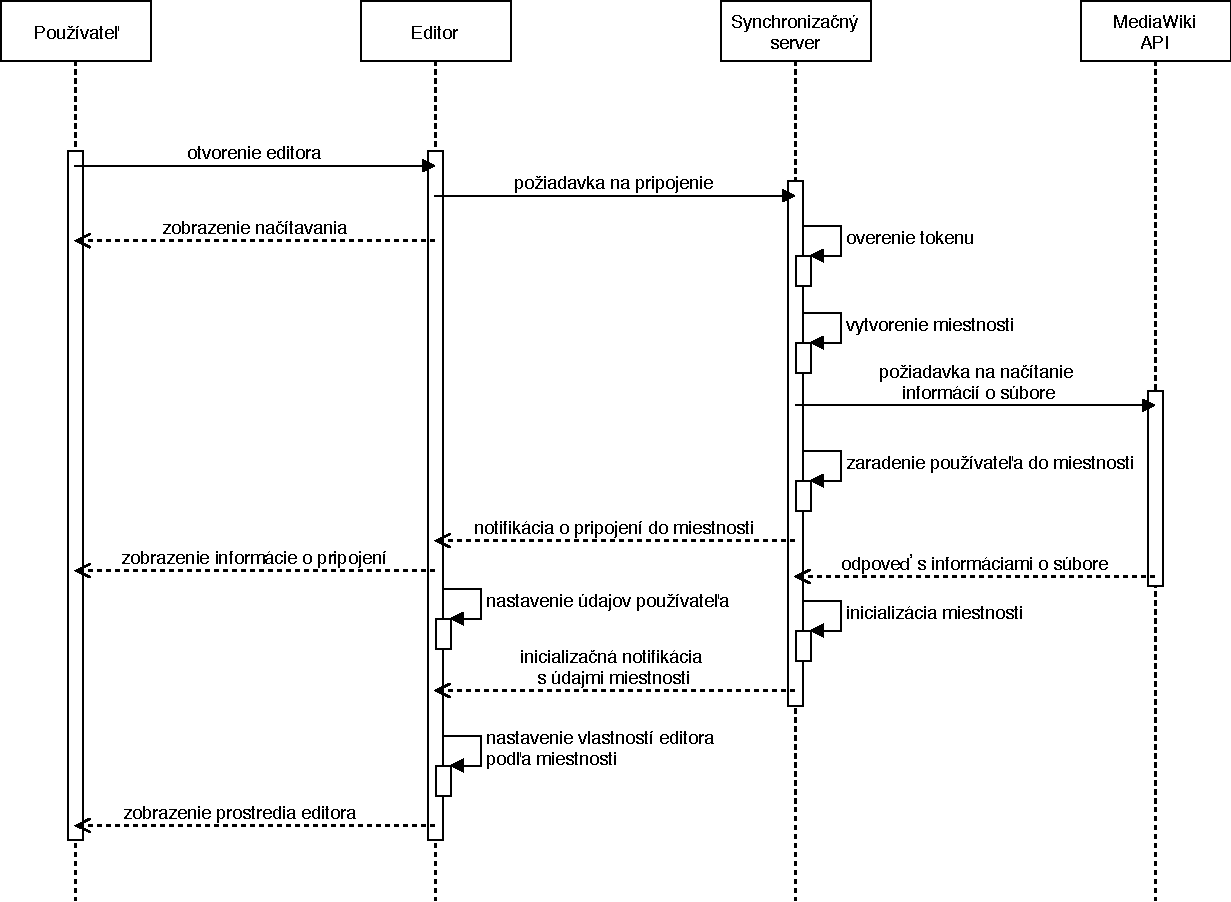
\includegraphics[width=1\textwidth]{images/diagrams/sequence-diagram-server-connect}}
	\caption[Sekvenčný diagram pripojenia používateľa]{Sekvenčný diagram úspešného pripojenia používateľa na synchronizačný server}
	\label{obr:sequence-diagram-server-connect}
\end{figure}
\FloatBarrier

\subsection{Spracovanie udalostí grafického editora}
S pripojením do miestnosti získava používateľ možnosť odosielať a prijímať synchronizačné správy. Synchronizačný server prijíma nasledujúce názvy udalostí:
\begin{itemize}
	
	\item \code{\'canvas-modified\'} -- \textit{Zmeny grafickej plochy} spracováva triedna metóda \code{room.modifyCanvas(properties, socket);}, ktorej parametrami sú objekt \code{properties}, obsahujúci vlastnosti zmenenej grafickej plochy editora a \code{socket} objekt odosielateľa. Po zmene vlastností plochy v rámci servera je odoslaná udalosť so zmenami všetkým ostatným používateľom.
	
	\item \code{\'object-created\'} -- \textit{Vytvorenie objektu} je spracované metódou \\\code{room.createObject(object, socket);}. Tá vytvorí nový záznam v zozname objektov editora, indexovaný podľa jedinečného identifikátora objektu a odošle udalosť na vytvorenie objektu všetkým ostatným používateľom.
	
	\item \code{\'selection-changed\'} -- \textit{Zmena uzamknutia objektu} sa vyhodnotí metódou \code{room.setSelectable(data.id, data.selectable, user, socket);}. Parametrami sú jedinečný identifikátor objektu, stav či má byť objekt uzamknutý alebo odomknutý a používateľ, ktorý vykonáva túto zmenu. V prípade že objekt nemôže byť uzamknutý z dôvodu, že už bol uzamknutý iným používateľom, odosielateľ obdrží udalosť o zakázaní označenia daného objektu. Inak sa nastaví hodnota uzamknutia a odošle sa ostatným používateľom.
	
	\item \code{\'object-modified\'} -- \textit{Modifikácia objektu} je spracovaná pomocou metódy \code{room.modifyObject(object, socket);}, ktorá vyhľadá objekt na základe jedinečného identifikátora v zozname objektov a nastaví jeho nové vlastnosti podľa vstupného parametra \code{object}. V prípade že objekt v zozname neexistuje, vytvorí ho. Funkcia ďalej odošle udalosť na modifikáciu objektu všetkým ostatným používateľom.
	
	\item \code{\'object-removed\'} -- \textit{Odstránenie objektu} zabezpečuje triedna metóda \code{room.removeObject(id, socket);}. Tá odstráni objekt s jedinečným identifikátorom podľa vstupného parametra zo zoznamu objektov miestnosti a odošle udalosť na odstránenie objektu ostatným používateľom.
	
	\item \code{\'message-created\'} -- \textit{Vytvorenie textovej správy} v chate editora je spracovaná metódou \\ \code{room.createMessage(message.text, message.from, message.to);}. Parameterami sú údaje prijaté v požiadavke, nesúce informácie o obsahu, odosielateľovi a prijímateľovi správy. Táto správa sa následne rozdistribuuje medzi všetkých používateľov pripojených do miestnosti.
	
\end{itemize}

\subsection{Odpojenie klienta}
Proces odpojenia používateľa pozostáva z jeho odstránenia zo zoznamu používateľov v miestnosti, zrušenia príznaku uzamknutého objektu všetkých objektov, ktoré mal používateľ pri odchode uzamknuté a odoslania udalosti všetkým zvyšným používateľom. Trieda \code{RoomManager} overí počet používateľov v miestnosti a pokiaľ zostala miestnosť prázdna, vymaže ju zo svojho zoznamu pomocou metódy \code{removeRoom(name);}.





\section{Grafický editor obrázkov}
Druhou časťou implementácie tejto diplomovej práce je naprogramovanie grafického editora obrázkov. Editor je implementovaný formou \textit{special page} rozšírenia, integrovaného do systému MediaWiki. Na vykresľovanie objektov grafickej plochy a udržiavanie jej stavu využívame knižnicu Fabric. Dátový model aplikácie je preto z veľkej časti závislý od dátového modelu tejto knižnice. Kolaboratívna funkcionalita je docielená použitím klientskej verzie Socket.IO knižnice, pomocou ktorej zabezpečujeme komunikáciu so synchronizačným serverom. Na riadenie klientského rozhrania používame knižnicu AngularJS. Komponenty používateľského prostredia sú naprogramované v šablónovacom jazyku HTML a ich vzhľad je naprogramovaný pomocou štýlovacieho jazyka LESS.

\subsection{MediaWiki rozšírenie}
Pri tvorbe rozšírení pre MediaWiki je potrebné dodržať základné návrhové konvencie stanovené tvorcami tohoto systému. Prvoradou vlastnosťou je jednoduchá inštalácia a nastavenie rozšírenia. To je docielené pomocou viacerých faktorov. Dôležité je používanie správnej súborovej štruktúry. 

Rozšírenie musí byť umiestnené vo vlastnom priečinku medzi ostatnými MediaWiki rozšíreniami. V našom prípade je to priečinok \code{/extensions/ImageEditor}, kde sa nachádzajú zdrojové súbory a priečinky kategorizované podľa ich obsahu. V priečinku \code{i18n} sa nachádzajú php súbory s prekladmi textov použitých v prostredí rozšírenia, nazvané skratkou jazyka, do ktorého sú preložené. Pre slovenčinu je to \code{sk.php}.

Zdrojový súbor \code{ImageEditor.php} zabezpečuje možnosť načítania rozšírenia pomocou príkazu \code{wfLoadExtension( \'ImageEditor\' );} v konfiguračnom súbore \code{LocalSettings.php}.

Súbor \code{ImageEditor.hooks.php} obsahuje funkcie, pomocou ktorých vieme odchytiť akcie vykonávané jadrom systému, a ovplyvniť tak jeho základnú funkcionalitu. V tomto súbore sa nachádza trieda \code{ImageEditorHooks} poskytujúca nasledujúce statické metódy:

\begin{itemize}
	\item \code{onFileUpload} -- funkcia odchytávajúca nahrávanie nového multimediálneho súboru alebo jeho novej revízie, pomocou ktorej uložíme obsah editora do metadát súboru. Metadáta sú uchovávané v databáze formou databázového dátového typu \code{blob}. Obsahom je serializované pole jazyka php. Naše rozšírenie pri ukladaní revízie zapíše do tohoto poľa svoju dátovú štruktúru serializovanú do JSON textového formátu, ktorá je odosielaná pri ukladaní súboru pomocou POST premennej HTTP dotazu, pod indexom \code{imageEditorContent}.
	
	\item \code{onSkinTemplateNavigation} -- metóda odchytáva proces vykreslenia navigačných tlačidiel pri vykreslení šablóny stránok. Na základe overenia práv používateľa a typu vykresľovanej stránky sa pridá tlačidlo na otvorenie súboru v našom editore obrázkov \refimg{obr:base-integration}.
	
	\item \code{onSkinTemplateNavigation_SpecialPage} -- podobná metóda ako \\
	\code{onSkinTemplateNavigation} s výnimkou, že táto udalosť je volaná pri vykresľovaní šablóny špeciálnych stránok.
	
	\item \code{onResourceLoaderGetConfigVars} -- metóda slúži na pridanie konfiguračných premenných posielaných do JavaScriptového rozhrania systému MediaWiki. Vďaka tomu môžeme pristupovať k premenným definujúcim bezpečnostný token, port a adresu synchronizačného servera z klientskej aplikácie naprogramovanej v jazyku JavaScript pomocou premenných 
	\begin{itemize}
		\item \code{mw.config.values.wgImageEditor.secret}
		\item \code{mw.config.values.wgImageEditor.host}
		\item \code{mw.config.values.wgImageEditor.port}
	\end{itemize}
\end{itemize}

V súbore \code{templates/ImageEditorTemplate.php} sa nachádza php trieda \\
\code{ImageEditorTemplate} dedená od triedy \code{QuickTemplate}, obsahujúca jednu metódu s názvom \code{execute()}. Volaním tejto metódy sa vykreslí HTML šablóna nášho rozšírenia.

Hlavná logika načítania rozšírenia sa však odohráva v triede \code{SpecialImageEditor}, umiestnenej v súbore \code{specials/SpecialImageEditor.php}. V metóde \code{execute()} sa vykoná overenie práv na upravovanie stránok a overí sa, či je vybraný súbor, ktorý chceme upravovať. Ak používateľ nemá práva na úpravu, je presmerovaný buď na prihlásenie (neprihlásený používateľ) alebo chybovú stránku.

Ak používateľ vytvára nový súbor pomocou adresy \\
\code{https://wiki.matfyz.sk/Special:ImageEditor} zobrazí sa mu formulár s výzvou na zadanie názvu súboru \refimg{obr:base-new}. Po jeho zadaní je presmerovaný do prostredia editora.

\begin{figure}[H]
	\centerline{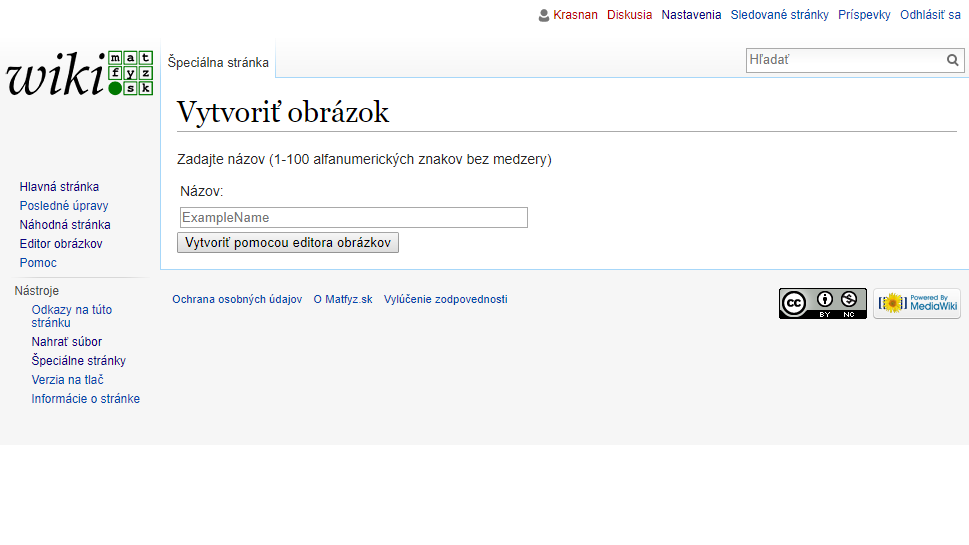
\includegraphics[width=1\textwidth]{images/results/base-new}}
	\caption{Používateľské prostredie na zadanie názvu nového obrázku.}
	\label{obr:base-new}
\end{figure}

\begin{figure}[H]
	\centerline{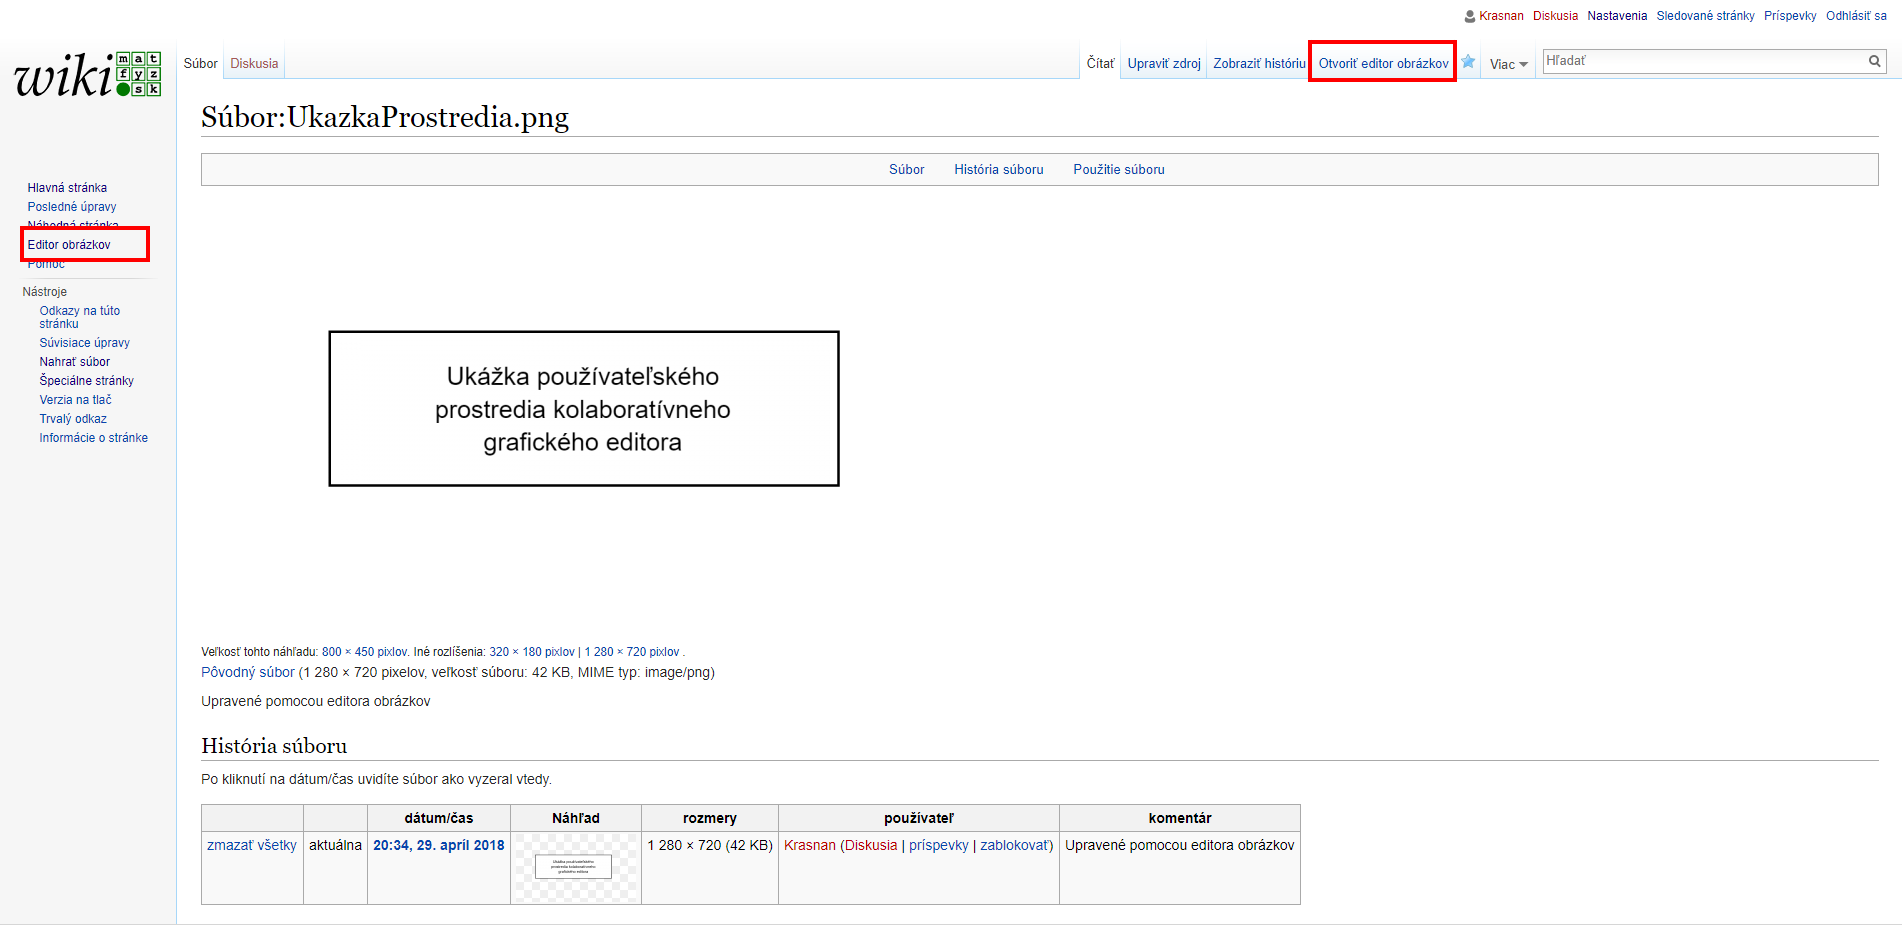
\includegraphics[width=1\textwidth]{images/results/base-integration}}
	\caption{Integrácia do natívneho prostredia systému MediaWiki.}
	\label{obr:base-integration}
\end{figure}


Zdrojové kódy editora naprogramované v jazyku JavaScript sú umiestnené v priečinku \code{resources/scripts}. Pre ich lepšiu prehľadnosť sme ich rozdelili do súborov podľa zamerania funkcií, ktoré obsahujú \reftab{tab:editor-scripts-files}. Kaskádové štýly používateľského prostredia editora sa nachádzajú v priečinku \code{resources/styles} a taktiež sú rozdelené podľa funkcionality \reftab{tab:editor-styles-files}. Použité knižnice sa nachádzajú v priečinku \code{resources/vendor} a zdrojové obrázky spolu s písmami v priečinku \code{resources/assets}.

\begin{table}
	\begin{tabular}{ | m{6cm} | m{6.5cm} | } \hline
		\textbf{Názov} & \textbf{Popis} \\ \hline \hline
		
		ext.imageEditor.utils.js & Definície globálnych funkcií a prototypovanie vlastných metód knižnice Fabric. \\\hline
		ext.imageEditor.init.databinding.js & Definície funkcií na prístup k premenným objektov knižnice Fabric pomocou Angular controlleru. \\\hline
		ext.imageEditor.init.tools.js & Definície funkcií na prácu s používateľským prostredím editora. \\\hline
		ext.imageEditor.init.events.js & Definície funkcií na riadenie udalostí (event-handlers) grafickej plochy a synchronizačných správ. \\\hline
		ext.imageEditor.init.keybindings.js & Definícia funkcie na spracovanie klávesových skratiek. \\\hline
		ext.imageEditor.init.history.js & Príprava pre funkcionalitu ukladania histórie zmien (undo, redo). \\\hline
		ext.imageEditor.init.app.js & Inicializácia Angular controllera, služby poskytujúcej prístup k funkciám knižnice Socket.IO a definícia direktív Angular modulu pre vytvorenie vlastných HTML elementov a atribútov. \\\hline
		
		\hline
	\end{tabular}
	\caption{Zoznam JavaScriptových zdrojových súborov editora}
	\label{tab:editor-scripts-files}
\end{table}

\begin{table}
	\begin{tabular}{ | m{6cm} | m{6.5cm} | } \hline
		\textbf{Názov} & \textbf{Popis} \\ \hline \hline
		
		ext.imageEditor.vars & Definície premenných, mixinov a dedičných tried. \\\hline
		ext.imageEditor.colorpicker & Štýly pre komponent vyberača farieb. \\\hline
		ext.imageEditor.icons & Definície premenných a tried pre ikony používateľského prostredia. \\\hline
		ext.imageEditor.less & Definície štýlov používateľského prostredia editora. \\\hline
		
		\hline
	\end{tabular}
	\caption{Zoznam LESS zdrojových súborov kaskádových štýlov}
	\label{tab:editor-styles-files}
\end{table}

Pri tvorbe rozšírenia pre systém MediaWiki je veľmi dôležitý súbor \\
\code{extension.json}, nachádzajúci sa v jeho koreňovom priečinku. Slúži na definovanie umiestnenia súborov, závislostí na iných rozšíreniach a ich automatického načítavania pomocou \textit{resource loaderu}.




\subsection{Aplikácia grafického editora}
Aplikácia grafického editora je naprogramovaná v jazyku JavaScript pomocou frameworku AngularJS. Všetky jej funkcie sú naprogramované v module s názvom \code{ImageEditor}. Modul poskytuje direktívy pre šablónu, ktoré zabezpečujú dynamické vykresľovanie niektorých používateľských komponentov, pridávajú im dodatočnú funkcionalitu, upravujú spôsob mapovania dát alebo poskytujú prístup k službám knižnice Socket.IO \reftab{tab:image-editor-directives}.
\begin{table}
	\begin{tabular}{ | m{4cm} | m{8.5cm} | } \hline
		\textbf{Názov} & \textbf{Popis} \\ \hline \hline
		
		\code{bindValueTo} & Direktíva na dynamické mapovanie get/set funkcií nastavujúcich hodnoty modelu Fabric objektov. Zabezpečuje zmenu modelu pri zmene hodnoty HTML vstupných elementov vykreslených šablónou editora. \\\hline
		\code{onEnter} & Direktíva, ktorá pridaním svojho atribútu do HTML vstupného elementu zabezpečuje volanie funkcií pri stlačení klávesy enter. \\\hline
		\code{filesInput} & Direktíva poskytuje funkciu načítania obrazového súboru, a následné mapovanie jeho hodnoty v textovom dataURI formáte do zvolenej premennej modelu aplikácie. \\\hline
		\code{socket} & Direktíva poskytujúca prístup k službám knižnice Socket.IO pomocou funkcie \code{$ \$ $scope.socket.on(\'event-name\', callback)}, odchytávajúce udalosti prichádzajúce zo synchronizačného servera, a funkcie \code{$ \$ $scope.socket.emit(\'event-name\', \{...\})}, odosielajúcej udalosti na synchronizačný server. \\\hline

		\hline
	\end{tabular}
	\caption{Zoznam direktív AngularJS modulu ImageEditor}
	\label{tab:image-editor-directives}
\end{table}

Okrem direktív modul obsahuje taktiež controller s názvom \\
\code{ImageEditorController}, riadiaci funkcionalitu a správanie grafického editora. Kvôli dostupnosti funkcií priamo v šablóne je potrebné všetky funkcie a premenné definovať do \code{$ \$ $scope} objektu. 

\subsubsection{Mapovanie dát}

Ako sme si vysvetlili v sekcii \ref{sec:angular}, Angular je navrhnutý tak, aby dokázal dynamicky zobrazovať hodnoty modelu v šablóne aplikácie pomocou dátového mapovania. Aby sme boli schopní mapovať dátový model Fabric canvas objektu, je potrebné naprogramovať metódy na prístup k jeho hodnotám. Musíme tak učiniť z dôvodu, že hodnoty modelu nie vždy zodpovedajú hodnotám, ktoré potrebujeme zobrazovať v používateľskom prostredí. Zdrojový súbor \code{ext.imageEditor.init.databinding.js} obsahuje funkcie určené na túto činnosť. Okrem funkcií popísaných v Tabuľke \ref{tab:editor-func-databinding}, sú v tomto súbore taktiež \code{set} a \code{get} funkcie definované pre každú premennú Fabric objektov \cite{FabricApiDoc}, ku ktorej je potrebné pristupovať z používateľského prostredia.

\begin{table}
	\begin{tabular}{ | m{7.5cm} | m{5cm} | } \hline
		\textbf{Názov} & \textbf{Popis} \\ \hline \hline
		
		\code{getActiveStyle(styleName, object)} & Funkcia na prístup k hodnote premennej štýlov \code{styleName} objektu \code{object} alebo aktívneho objektu.\\\hline
		\code{setActiveStyle(styleName, value, object)} & Funkcia na nastavenie premennej štýlu \code{styleName} hodnotou \code{value} objektu \code{objekt} alebo aktívneho objektu.\\\hline
		\code{getActiveProp(name)}  & Funkcia na prístup k hodnote \code{name} premennej aktívneho objektu. \\\hline
		\code{setActiveProp(name, value)}  & Funkcia na nastavenie premennej \code{name} hodnotou \code{value} aktívneho objektu. \\\hline
		
		\hline
	\end{tabular}
	\caption{Zoznam základných funkcií nastavujúcich hodnoty modelu Fabric objektov}
	\label{tab:editor-func-databinding}
\end{table}

\subsubsection{Riadenie udalostí (Event-handler)}
Naša aplikácia využíva princípy programovania riadeného udalosťami (event-driven). Dokáže dynamicky vyhodnocovať niektoré z udalostí, ktoré sa v nej vykonávajú, bez potreby volania funkcií spracovávajúcich danú akciu do častí kódu, kde je daná akcia vykonávaná. Namiesto toho sa použije funkcia \code{$\$$scope.canvas.trigger(\'event-name\', {...})}, pomocou ktorej sa vyvolá udalosť s názvom podľa prvého parametra a dátami uloženými v druhom parametri tejto funkcie. Následne je možné tieto udalosti jednoducho zachytiť v našej aplikácií. 

Okrem akcií grafickej plochy spracovávame taktiež udalosti vyvolávané synchronizačnými správami servera, poskytované službami knižnice Socket.IO. Zoznam a popis udalostí, ktoré naša aplikácia dokáže spracovať, môžeme vidieť v tabuľkách \reftab{tab:editor-events} a \reftab{tab:server-events}.

\begin{table}
	\begin{tabular}{ | m{4cm} | m{8.5cm} | } \hline
		\textbf{Názov} & \textbf{Popis} \\ \hline \hline
		
		object:created & Vytvorenie nového grafického objektu. Odosiela sa požiadavka synchronizačnému serveru na vytvorenie nového objektu. \\\hline
		object:modified & Zmena grafického objektu. Odosiela sa požiadavka synchronizačnému serveru na modifikáciu objektu. \\\hline
		object:removed & Odstránenie grafického objektu. Odosiela sa požiadavka synchronizačnému serveru na vymazanie objektu.  \\\hline
		object:moving & Pohyb objektu pomocou kurzora použivateľa. Ak je zapnuté prichytávanie k mriežke, hodnoty pozície pohybovaného objektu sa nastavia na zaokrúhlené číslo v závislosti od veľkosti priblíženia grafickej plochy.  \\\hline
		path:created & Vytvorenie nového grafického objektu počas voľného kreslenia. Odosiela sa požiadavka synchronizačnému serveru na vytvorenie nového objektu. \\\hline
		canvas:modified & Zmena vlastností grafickej plochy. Odosiela sa požiadavka synchronizačnému serveru na zmenu grafickej plochy. \\\hline
		selection:created, selection:updated, selection:cleared & Zmena označenia aktívneho objektu. Odosielajú sa požiadavky synchronizačnému serveru na zmenu uzamknutia objektov, ktorých sa zmena týka. \\\hline
		mouse:over & Nadídenie kurzorom nad objekt. Ak je objekt uzamknutý, zobrazí sa v grafickej ploche meno používateľa, ktorý ho uzamkol. \\\hline
		mouse:out & Odídenie kurzorom z objektu grafickej plochy. Ak je zobrazené meno používateľa nad objektom, skryje sa. \\\hline
		
		\hline
	\end{tabular}
	\caption{Zoznam udalostí grafickej plochy}
	\label{tab:editor-events}
\end{table}

\begin{table}
	\begin{tabular}{ | m{4cm} | m{8.5cm} | } \hline
		\textbf{Názov} & \textbf{Popis} \\ \hline \hline
		
		connected & Pripojenie na synchronizačný server. Nastaví sa objekt pripojeného používateľa a skryje sa správa o pripájaní v loaderi. \\\hline
		init & Inicializačná správa s informáciami, podľa ktorých sa nastavuje editor. Pridajú sa všetky objekty do grafickej plochy, vytvorí sa zoznam pripojených používateľov, načíta sa zoznam správ a nastavia sa vlastnosti grafickej plochy. \\\hline
		user-created & Pripojenie nového používateľa do miestnosti. Používateľ je pridaný do zoznamu všetkých používateľov. \\\hline
		user-removed & Odpojenie používateľa z miestnosti. Používateľ je odstránený zo zoznamu všetkých používateľov. \\\hline
		message-created & Prijatá nová správa. Nastaví sa príznak na zobrazenie notifikácie o novej správe a obsah správy sa zaradí do zoznamu správ. \\\hline
		selection-changed & Zmena uzamknutia objektu. Nastaví sa hodnota \code{selectable} a \code{selectedBy} podľa prijatej správy, čím sa zamedzí možnosti označiť daný objekt. \\\hline
		object-created & Vytvorenie objektu. Objekt prijatý v správe sa pridá do grafickej plochy. Ak objekt s daným identifikátorom existuje, proces sa ukončí. \\\hline
		object-modified & Modifikácia objektu. Na základe vlastností objektu prijatého v správe sa nastavia vlastnosti objektu s relevantným identifikátorom v grafickej ploche editora. Ak objekt s daným identifikátorom neexistuje, vytvorí sa, čím zabezpečíme nápravu prípadnej straty alebo výrazného oneskorenie správy o vytvorení objektu. \\\hline
		object-removed & Odstránenie objektu. Na základe prijatého identifikátora sa odstráni objekt z grafickej plochy. \\\hline
 		canvas-modified & Zmena vlastností grafickej plochy. Nastavia sa vlastnosti na základe prijatých informácií. \\\hline
		   
		\hline
	\end{tabular}
	\caption{Zoznam udalostí synchronizačného servera}
\label{tab:server-events}
\end{table}
\FloatBarrier
\subsubsection{Používateľské prostredie}
Používateľské prostredie editora je nadizajnované tak, aby bola každá funkcionalita prístupná pokiaľ možno na jedno kliknutie používateľa. Pozostáva zo 4. hlavných komponentov.

\begin{figure}[H]	
	\centerline{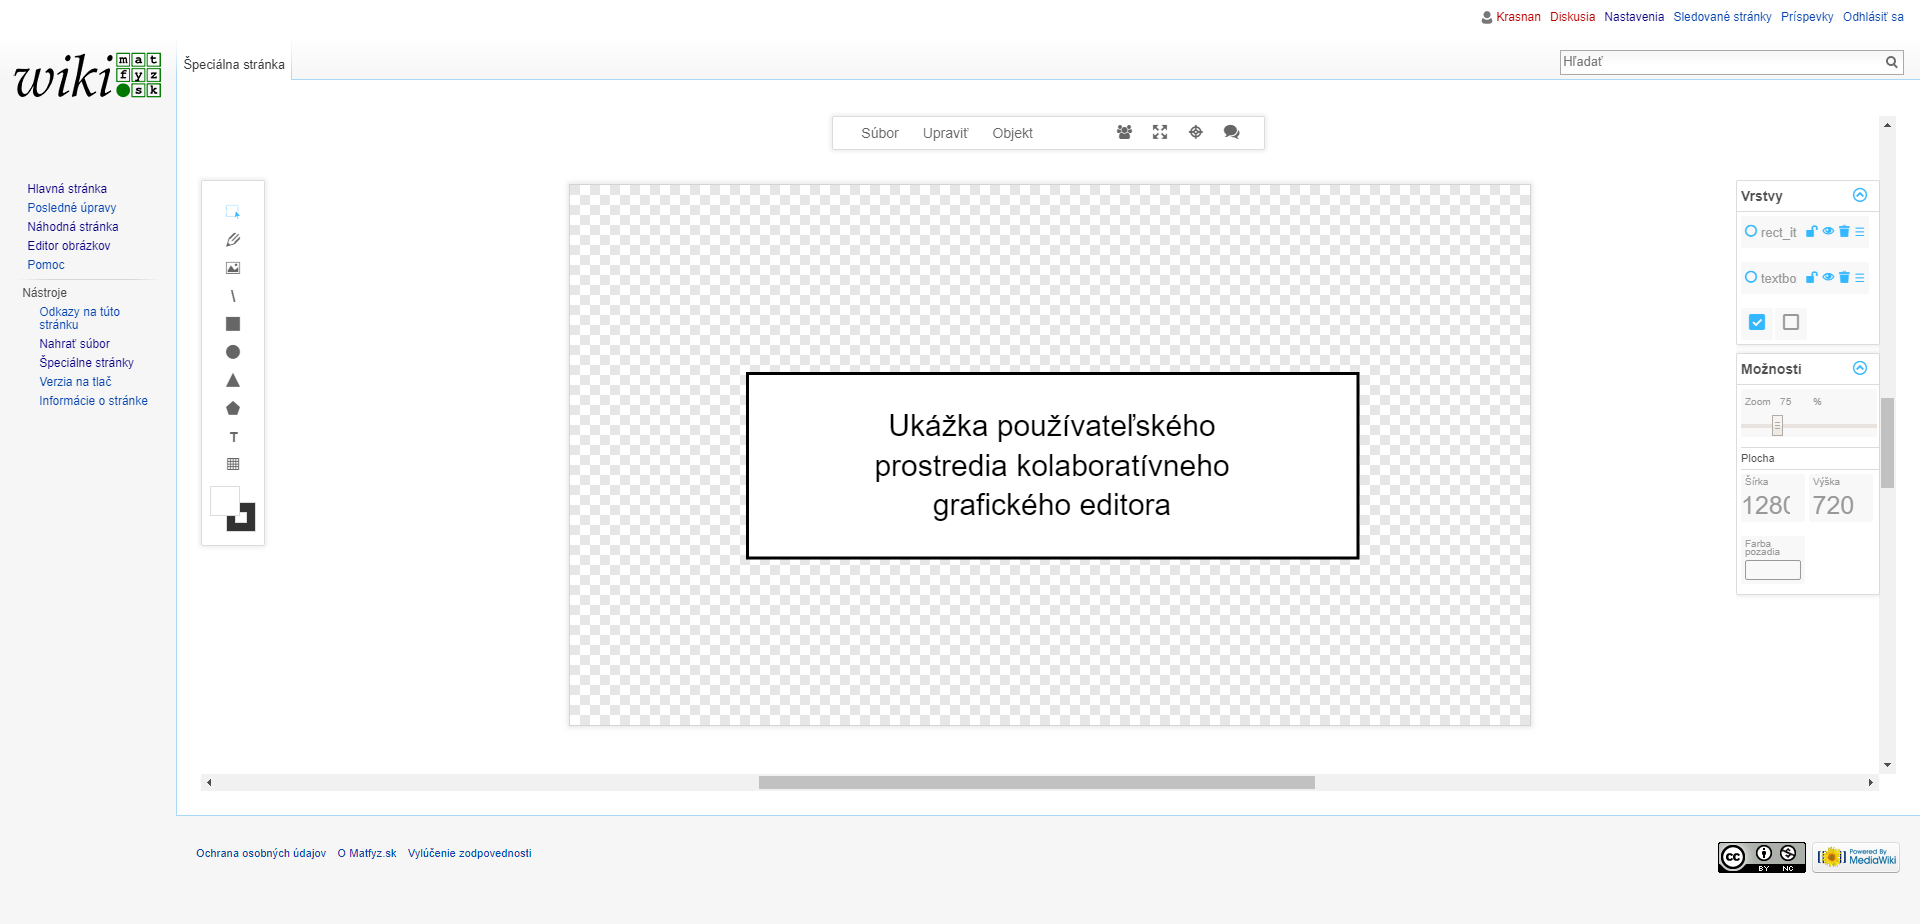
\includegraphics[width=1\textwidth]{images/results/base-editor}}
	\caption{Používateľské prostredie grafického editora obrázkov.}
	\label{obr:base-user-interface}
\end{figure}
	
\textbf{Grafická plocha}, v ktorej sú vykresľované jednotlivé grafické objekty. Ak je niektorý z objektov uzamknutý iným používateľom, prístup k tomuto objektu bude zamietnutý. Pri nadídení kurzora počítačovej myši sa zobrazí meno používateľa používajúceho daný objekt \refimg{obr:canvas-locked}.
\begin{figure}[H]
	\centering
	\begin{subfigure}[t]{0.48\linewidth}	
		\centering{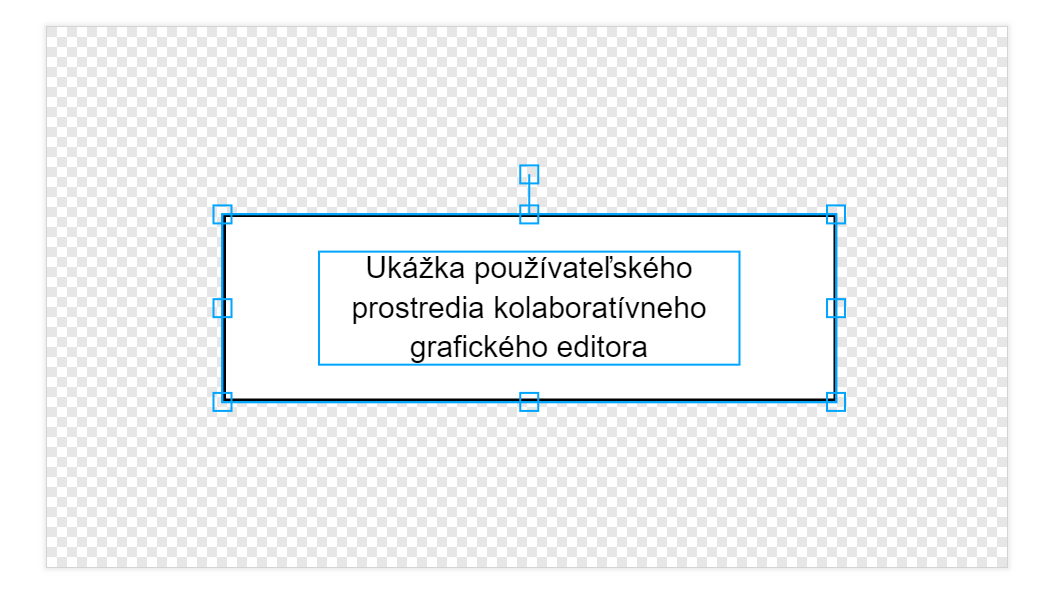
\includegraphics[width=1\textwidth]{images/results/canvas-selected}}
		\caption{Označenie aktívnych objektov}
		\label{obr:canvas-selected}
	\end{subfigure}
	\quad
	\begin{subfigure}[t]{0.48\linewidth}	
		\centering{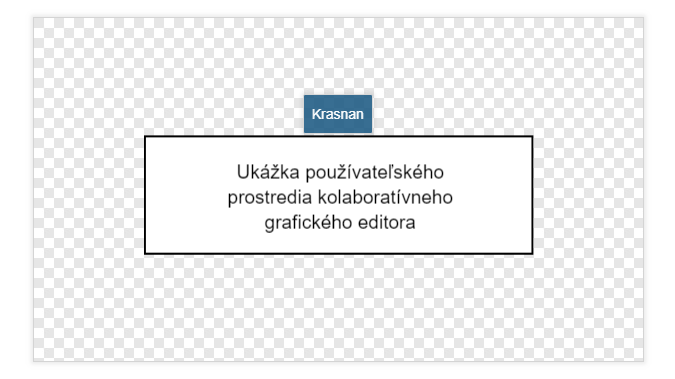
\includegraphics[width=1\textwidth]{images/results/canvas-locked}}
		\caption{Zobrazenia používateľa, ktorý uzamkol objekt}
		\label{obr:canvas-locked}
	\end{subfigure}
	
	\caption{Grafická plocha edit}
\end{figure}

 \textbf{Panel nástrojov} s tlačidlom pre každý nástroj a tlačidlami pre výber farby výplne a obtiahnutia objektu. V paneli sa taktiež nachádza tlačidlo na zapnutie prichytávania objektov k mriežke grafickej plochy.
	
\begin{figure}[H]
	\centering
	\begin{subfigure}[t]{0.48\linewidth}	
		\centering{
\includegraphics[height=6cm]{images/results/toolbar}}
		\caption{Zoznam nástrojov grafického editora}
	\end{subfigure}
	\quad
	\begin{subfigure}[t]{0.48\linewidth}	
		\centering{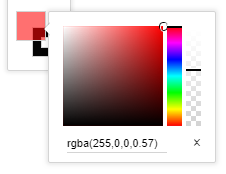
\includegraphics[height=5cm]{images/results/toolbar-colorpicker}}
		\caption{Vyberač farby výplne a obtiahnutia objektu grafickej plochy}
	\end{subfigure}
	\caption{Panel nástrojov}
\end{figure}



\textbf{Hlavné menu} obsahujúce tlačidlo na prepnutie zobrazenia do režimu celej obrazovky, tlačidlo na vycentrovanie grafickej plochy a rozbaľovací zoznam správ chatu \refimg{obr:menu-messenger}. Okrem týchto tlačidiel tu nájdeme aj 3 rozbaľovacie (dropdown) tlačidlá \textit{Súbor} , \textit{Upraviť} a \textit{Objekt}. Rozbalením tlačidla \textit{Súbor} \refimg{obr:menu-file} sa zobrazí ponuka na exportovanie grafickej plochy do formátov PNG a SVG, uloženie revízie a zatvorenie editora. Rozbalením tlačidla \textit{Upraviť} \refimg{obr:menu-edit} sa sprístupnia možnosti na kopírovanie, vystrihnutie, vloženie, duplikovanie a odstránenie objektu. Pod posledným tlačidlom \textit{Objekt} \refimg{obr:menu-object}, sa zobrazia možnosti operácií s aktívnym objektom na zmenu hĺbky objektu v grafickej ploche.
\begin{figure}[H]
	\centering
	\begin{subfigure}[t]{0.48\linewidth}	
		\centering{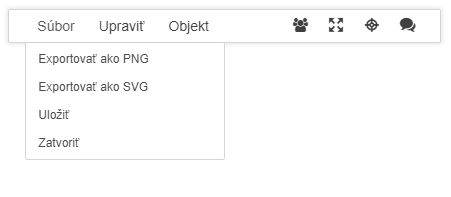
\includegraphics[width=1\textwidth]{images/results/menu-file}}
		\caption{Rozbaľovacie menu pre tlačidlo \textit{Súbor}}
		\label{obr:menu-file}
	\end{subfigure}
	\quad
	\begin{subfigure}[t]{0.48\linewidth}	
		\centering{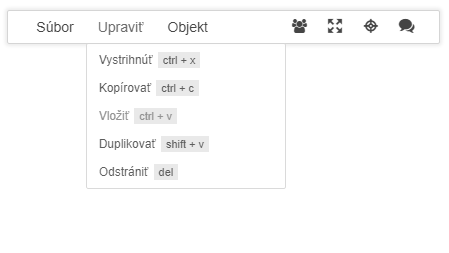
\includegraphics[width=1\textwidth]{images/results/menu-edit}}
		\caption{Rozbaľovacie menu pre tlačidlo \textit{Upraviť}}
		\label{obr:menu-edit}
	\end{subfigure}
	\quad
	\begin{subfigure}[t]{0.48\linewidth}	
		\centering{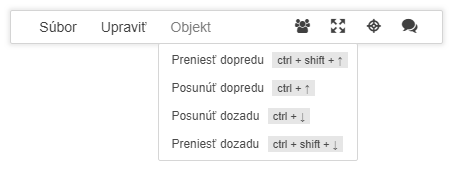
\includegraphics[width=1\textwidth]{images/results/menu-object}}
		\caption{Rozbaľovacie menu pre tlačidlo \textit{Objekt} }
		\label{obr:menu-object}
	\end{subfigure}
	\quad
	\begin{subfigure}[t]{0.48\linewidth}	
		\centering{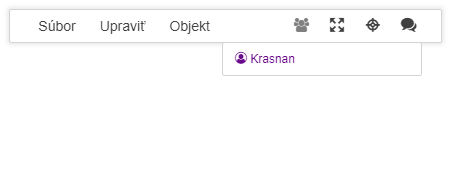
\includegraphics[width=1\textwidth]{images/results/menu-users}}
		\caption{Rozbaľovacie menu zoznamu pripojených používateľov  }
		\label{obr:menu-users}
	\end{subfigure}
	\quad
	\begin{subfigure}[t]{0.6\linewidth}	
		\centering{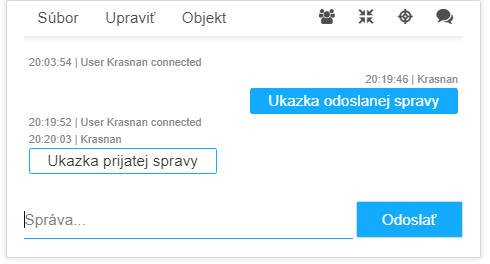
\includegraphics[width=1\textwidth]{images/results/menu-messenger}}
		\caption{Prostredie pre odosielanie textových správ}
		\label{obr:menu-messenger}
	\end{subfigure}
	\caption{Zobrazenie hlavného menu}
\end{figure}

\newpage
	
\textbf{Panel nastavení} tvorený dvoma komponentmi. Komponent vrstiev zobrazujúci zoznam všetkých grafických objektov s možnosťou ich rýchleho uzamknutia, skrytia a odstránenia. Vrstvy môžu byť preusporiadané pomocou ťahania kurzora, čím sa mení ich hĺbka v grafickej ploche editora. Druhý komponent obsahujúci nastavenia aktuálneho kontextu editora dynamicky zobrazuje položky na nastavenie vlastností aktívneho objektu, grafickej plochy, alebo nastavenia voľného kreslenia \refimg{obr:props}.
\begin{figure}[H]
	\centering
	\begin{subfigure}[t]{0.3\linewidth}	
		\centering{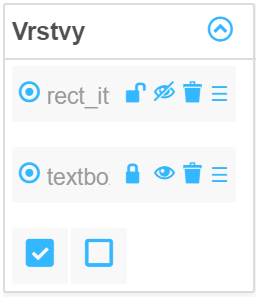
\includegraphics[height=4cm]{images/results/props-layers}}
		\caption{Panel vrstiev }
		\label{obr:props-layers}
	\end{subfigure}
	\quad
	\begin{subfigure}[t]{0.3\linewidth}	
		\centering{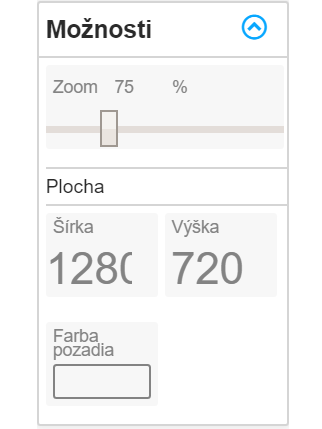
\includegraphics[height=4cm]{images/results/props-canvas}}
		\caption{Panel nastavení grafickej plochy}
		\label{obr:props-canvas}
	\end{subfigure}
	\quad
	\begin{subfigure}[t]{0.3\linewidth}	
		\centering{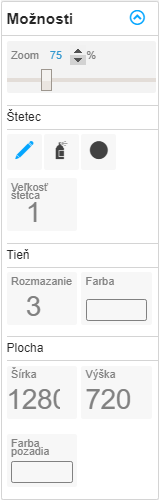
\includegraphics[height=4cm]{images/results/props-brush}}
		\caption{Panel nastavení voľného kreslenia}
		\label{obr:props-brush}
	\end{subfigure}
	\quad
	\begin{subfigure}[t]{0.48\linewidth}	
		\centering{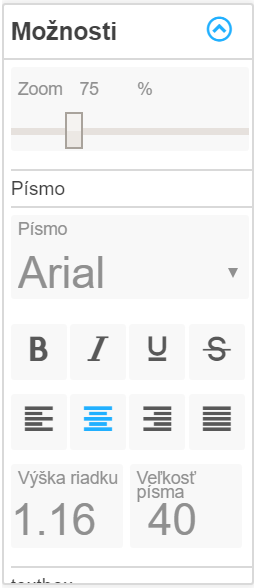
\includegraphics[height=5cm]{images/results/props-text}}
		\caption{Panel nastavení textového objektu}
		\label{obr:props-text}
	\end{subfigure}
	\quad
	\begin{subfigure}[t]{0.48\linewidth}	
		\centering{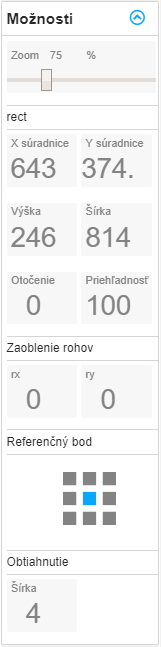
\includegraphics[height=5cm]{images/results/props-object}}
		\caption{Panel nastavení objektu}
		\label{obr:props-object}
	\end{subfigure}
	\caption{Ukážka panelov s nastaveniami}
	\label{obr:props}
\end{figure}
	


Okrem týchto panelov je potrebné informovať používateľa o niektorých vykonávaných akciách formou dialógových (\textit{popup}) správ s možnosťou potvrdenia alebo prípadného zrušenia akcie. Obsah dialógových okien je potrebné dynamicky vytvárať a modifikovať funkcionalitu potvrdzovacích tlačidiel. Využijeme ich na upozornenie používateľa pri odstraňovaní objektu z grafickej plochy \refimg{obr:editor-dialog-delete} a zatváraní okna editora, kde bude používateľ vyzvaný na uloženie súboru alebo ukončenie bez ukladania zmien \refimg{obr:editor-dialog-close}. Pomocou dialógového okna je taktiež riešené nahratie obrázku z lokálneho úložiska používateľa \refimg{obr:editor-dialog-upload}.

\begin{figure}[H]
	\centering
	\begin{subfigure}[t]{0.48\linewidth}	
		\centering{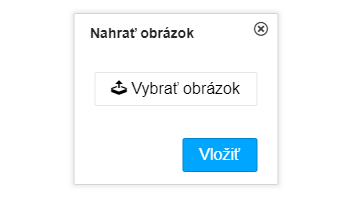
\includegraphics[width=1\textwidth]{images/results/dialog-upload}}
		\caption{Dialógové okno na nahratie súboru}
		\label{obr:editor-dialog-upload}
	\end{subfigure}
	\quad
	\begin{subfigure}[t]{0.48\linewidth}	
		\centering{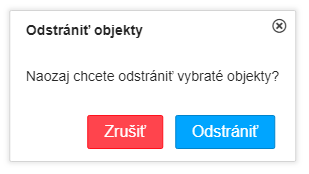
\includegraphics[width=1\textwidth]{images/results/dialog-delete}}
		\caption{Dialógové okno na potvrdenie vymazania grafického objektu}
		\label{obr:editor-dialog-delete}
	\end{subfigure}
	\quad
	\begin{subfigure}[t]{0.7\linewidth}	
		\centering{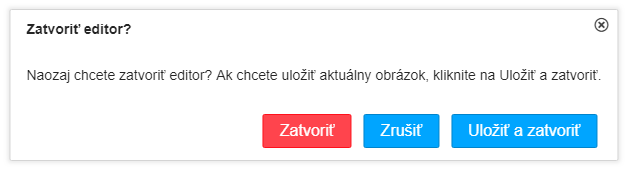
\includegraphics[width=1\textwidth]{images/results/dialog-close}}
		\caption{Dialógové okno zobrazené pri zatváraní editora}
		\label{obr:editor-dialog-close}
	\end{subfigure}
	\caption{Dialógové okná}
\end{figure}
\FloatBarrier